\chapter{Template considerations}

As you can see, the template handles the style of headings and spacing before and after them:

\section{Example section}
\subsection{Example subsection}
\subsubsection{Example subsubsection}
Lorem ipsum dolor sit amet, consectetur adipiscing elit. Cras quis nibh eu nunc consectetur tincidunt. Sed mauris turpis, dictum in sapien vel, porta rutrum ex.

\section{Figures and tables}

These can be generated as follows (\cref{fig:graph,tab:example}):

\begin{figure}[hbtp!]
    \centering
    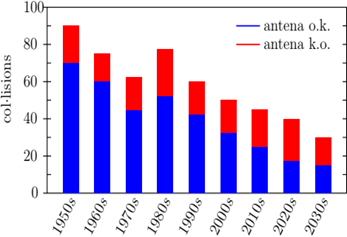
\includegraphics[width=0.5\linewidth]{img/example.png}
    \caption[Shorter name for list of tables or to escape the citation]{Caption below the image \cite{dawson}.}
    \label{fig:graph}
\end{figure}

Phasellus venenatis leo vitae sagittis aliquam. Fusce fringilla fringilla pharetra. Maecenas ac libero nec augue feugiat consectetur. Suspendisse potenti. Integer eget enim tincidunt risus aliquam dignissim in nec sem. Suspendisse ultrices hendrerit fringilla. Duis in nibh venenatis, blandit diam id, feugiat nisi. Mauris fermentum maximus dui nec accumsan. 

\begin{table}[htbp!]
    \centering
    \renewcommand{\arraystretch}{1.07}
    \begin{tabular}{@{}lccr@{}}
        \toprule
        \bfseries Dècada & \bfseries Antena ok & \bfseries Antena ko & \bfseries Total\\
        \midrule
        1950s & 70 & 20 & 90\\
        1960s & 60 & 18 & 78\\
        1970s & 44 & 21 & 63\\
        \bottomrule
    \end{tabular}
    \caption[Shorter name]{Caption below the table.}
    \label{tab:example}
\end{table}

\section{Bibliography}

The UPC recommends using the IEEE style, which this template uses. This is achieved with the \verb+biblatex+ and \verb+biblatex-ieee+ packages. Add your sources to \verb+references.bib+ following the biblatex scheme with whatever fields, and the style will determine which ones to show.

Most journal publishers feature a button to export the citation to BibTeX, usually under ``Cite" (e.g., ScienceDirect) or ``Tools" (e.g., Wiley). In that case, you can just copy the content of the .bib file to \verb+references.bib+. If there is no button or you aren't referencing a journal article, use the usual biblatex syntax.

In order to follow the \href{https://journals.ieeeauthorcenter.ieee.org/wp-content/uploads/sites/7/IEEE_Reference_Guide.pdf}{IEEE style} more closely, do the following:

\begin{outline}
    \1 If the reference has a DOI number, use the \verb+doi+ field in favor of the \verb+url+ field (i.e., delete the latter).
    \1 If the reference is recorded in a database that uses HDL, you can cite it like so:
    \2[] \verb+eprinttype = {hdl}, eprint={XXXXX/XXX}+
    \1 If a journal uses article numbers instead of pages, use the field \verb+eid+ instead:
    \2[] \verb+eid = {XXX}+
    \1 References to Bachelor's and Master's theses can be generated with the \verb+@mastersthesis+ entry type; remember to set the \verb+type+ to \verb+B.S. thesis+ or \verb+M.S. thesis+ accordingly.
    PhD dissertations are usually cited as \verb+@phdthesis+. 
    \1 The IEEE style calls for article or book titles to be in sentence case, that is, only the first letter of the title and proper names. However, the \LaTeX\ implementation converts them to lowercase indiscriminately; you can prevent this by surrounding the affected word with curly brackets \verb+{}+.
\end{outline}

Examples:
\begin{outline}
    \1[] Yada yada yada \cite{incollection}; \textcite{articlelargepages} stated that...; this has solid evidence \cite{dawson,ieec,bookwitheditor}. \nocite{Li2007}
\end{outline}

\section{Code listings and algorithms}

The EETAC style guide gives no direction on formatting algorithms, code snippets, or listings, so I took some liberties without straying much from the general style. Therefore, you can tweak these as you like.

{\centering
\begin{minipage}{.7\linewidth}
    \begin{algorithm}[H]
        \begin{algorithmic}[1]
            \Procedure{Euclid}{$a,b$}\Comment{The g.c.d. of a and b}
            \State $r\gets a\bmod b$
            \While{$r\not=0$}\Comment{We have the answer if r is 0}
            \State $a\gets b$
            \State $b\gets r$
            \State $r\gets a\bmod b$
            \EndWhile\label{euclidendwhile}
            \State \textbf{return} $b$\Comment{The gcd is b}
            \EndProcedure
        \end{algorithmic}
        \caption{Euclid's algorithm}
        \label{euclid}
    \end{algorithm}
\end{minipage}
\par
}

\begin{listing}[htbp!]
    \label{code:example}
    \inputminted[]{python}{img/example.py}
    \captionof{listing}{Some example code} 
\end{listing}